% Chapter Template

\chapter{Conclusiones} % Main chapter title

\label{Chapter5} % Change X to a consecutive number; for referencing this chapter elsewhere, use \ref{ChapterX}


%----------------------------------------------------------------------------------------

%----------------------------------------------------------------------------------------
%	SECTION 1
%----------------------------------------------------------------------------------------
En esté capítulo se presentan las conclusiones principales sobre la fabricación de un equipo dip coater, se detallan los logros más importantes del trabajo y se mencionan algunos puntos para mejorar en futuros desarrollos. Por último se plantean los planes inmediatos de desarrollo, fabricación y comercialización del equipo.

\section{Resultados obtenidos }


El principal hito del trabajo fue fabricar un MVP de equipo dip coater que cuanta con las características suficientes para satisfacer las demandas de primeros usuarios. 
Se señalan a continuación los siguientes logros en el desarrollo del presente trabajo: 
\begin{itemize}
\item Diseño y fabricación de un lote de cinco unidades con la primera versión de placa electrónica.
\item Desarrollo de un firmware modular que cumple con todos los requerimientos y permite incorporar nuevas funcionalidades sin cambios importantes en la estructura.
\item Generación de capacidad técnica suficiente para la fabricación de piezas mecanizadas del primer equipo.  
\end{itemize} 
 

Lamentablemente la planificación original no pudo ser sostenida. Abarcar íntegramente la fabricación de un MVP implicó demasiado trabajo para los tiempos y recursos establecidos. Existieron retrasos en el diseño y la fabricación mecánica que llevó a no poder estimar con exactitud los tiempos. Sin embargo, surge de este trabajo una base de conocimiento importante que permite comenzar con el desarrollo y la fabricación de otro MVP en tiempos más acotados y con una planificación más certera. 


%----------------------------------------------------------------------------------------
%	SECTION 2
%----------------------------------------------------------------------------------------
\section{Próximos pasos}

Se plantean los siguientes puntos fundamentales para el futuro inmediato del equipo:  

\begin{itemize}

\item Se fabricará un lote nuevo de diez placas incorporando los cambios mencionados en la sección \ref{section:Hardware}. 

\item Se incorporará un módulo de software para controlar parámetros de humedad, que será integrado con el desarrollo futuro de una cámara de humedad compatible con este equipo.

\item Durante el mes de octubre del presente año, investigadores del INS (Instituto de Nanositemas) llevarán a cabo ensayos para caracterizar el equipo. El ensayo contemplará la generación de cincuenta \textit{thin films} sobre soluciones químicas de \ce{TiO2} y \ce{SiO2} caracterizadas a través del método XRR (reflectometría de rayos-X). Surgirá de este ensayo un documento técnico con los resultados obtenidos.  
 
\item A través de un arreglo de cooperación se entregarán dos equipos a usuarios calificados para realizar pruebas funcionales y evaluar su satisfacción. Se realizarán cambios de ser necesario.


\item Se trabaja en conjunto con un diseñador industrial para convertir este MVP en un producto comercial de la empresa TECSCI, el la figura \ref{fig:new_dip} se observa el diseño que se está evaluando fabricar.


\begin{figure}[h!]
	\centering
	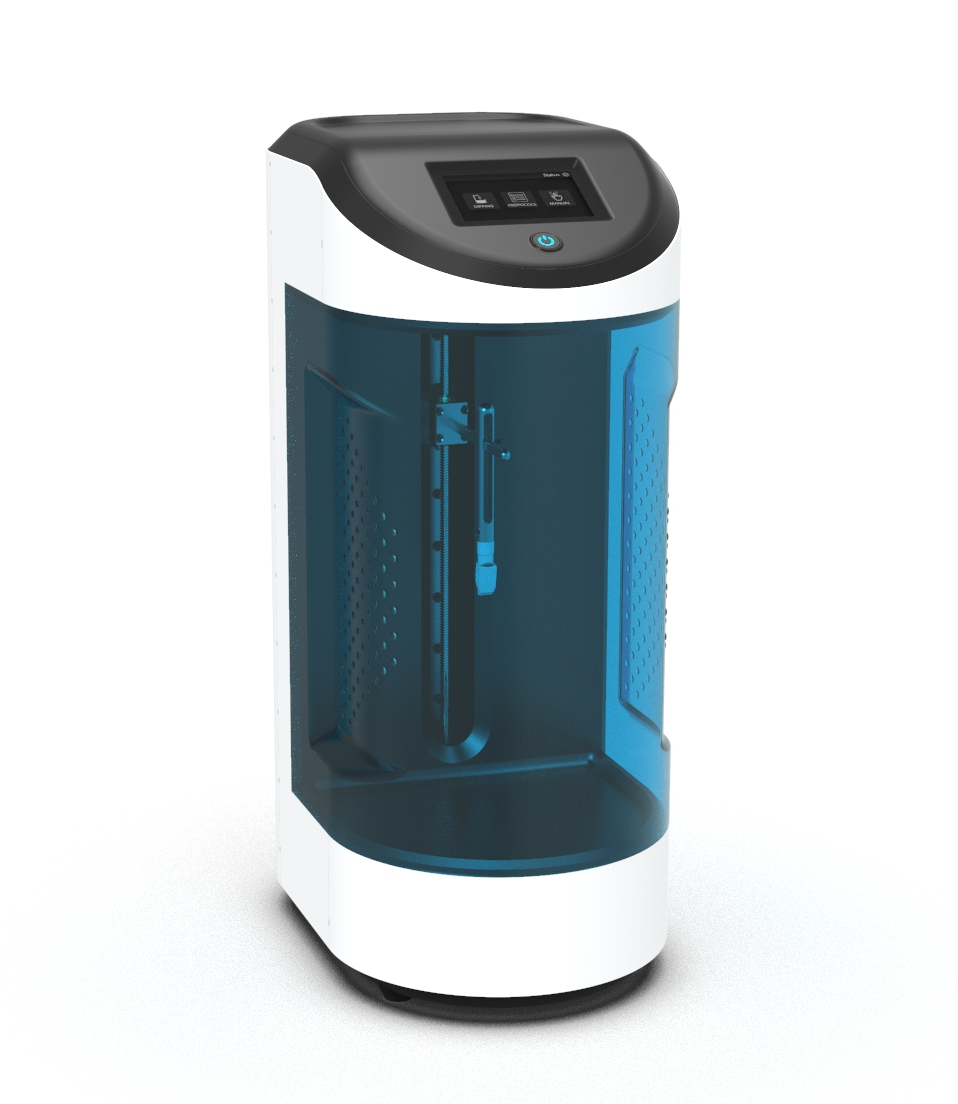
\includegraphics[width=0.95\textwidth]{./Figures/new_dip.png}
	\caption{Render de equipo comercial.}
	\label{fig:new_dip}
\end{figure}

\end{itemize}


